\documentclass{TDP003mall}
\usepackage{float}
\usepackage{listings}
\usepackage{graphicx}
\usepackage{hyperref}
\usepackage{parskip}
\usepackage{tabularx}
\usepackage{ltxtable}


\newcommand{\version}{Version 2.60}
\author{Arturas Alekandrausaksa,(NI)Chirster Vesterlund, Benjemin Graf, Vidar Wesrfelt, Gustav P Svensson, Dylan Mäenpää, Denis I. Blazevic, Alexander Jonsson, Deniz Ayar, Vera Antonov, Sokrates Lamprou, Niko Lehto, Albin Vedin, Adam Sterner, Mats Johansson, Jesper Olofsson, David Hilm, Viktor Brandt, David Rahim, Frans Bergström, Carl Lorentsson, Joakim Johansson, Erik Westerlund, Love Bäckman}
\title{Installationsmanual för Portföljsystem}
\date{2016-09-19}
\rhead{IP1 2016}

\begin{document}
\projectpage
\section{Revisionshistorik}
\LTXtable{\textwidth}{revisionshistorik.tex}


\section{Installera verktyg}
För att komma igång behöver du se till att du har verktygen \verb|python3|, \verb|Pip|, \verb|Flask| och \verb|Jinja2|.


Python är ett programmeringsspråk som du behöver installera för att kunna använda Flask och Jinja2 medan Pip är den pakethanterare som vi behöver för att kunna installera de två paketen. 
Flask är ett mikroramverk för webbutveckling som även har en inbyggd webbserver funktion som man kan använda medans utveckling av portföljsystem pågår. 
Tillsammans med Flask tillkommer Jinja2 templating. Jinja2 är ett modernt mall-språk för Python och används för att generera html output som skickas till användaren. Detta betyder att du inte måste uppdatera html-kod för varje gång du ska ladda upp något nytt på din sida, utan det löser Jinja2. 
Innan du påbörjar processen av att installera de paket som behövs kan det vara bra att se till att alla de paket du redan har installerade är uppdaterade.

Detta gör du enkelt genom att i terminalen skriva in:

\begin{lstlisting}[language=bash]
$ sudo apt-get update
\end{lstlisting}

\subsection{Installera Python 3}
\subsubsection{Vilken version har vi?}
Python 3 kan installeras antingen som \verb|python| eller \verb|python3|.
Python 3 finns oftast förinstallerat på systemet som \verb|python3|. Kolla vilka versioner du har. Använd den som motsvarar senaste versionen av Python 3:

\begin{lstlisting}[language=bash]
 $ python -V
 > Python 2.7.12
 $ python3 -V
 > Python 3.5.2
\end{lstlisting}

Om ditt resultat ser ut som ovan, använd framöver \verb|python3|. Vi kommer att skriva \verb|python3| i resten av manualen, men om du har Python 3 installerat som \verb|python|, använd den i stället.
\subsubsection{Linux}
Om Python 3 saknas så rekommenderas installation med hjälp av din distributions pakethanterare (i Linux Mint är detta \verb|apt-get|):



Linux Mint eller Ubuntu (python3 ska vara förinstallerat):
\begin{lstlisting}[language=bash]
$ sudo apt-get python3
\end{lstlisting}
Arch-Linux (python3 är standard i Arch-Linux):
\begin{lstlisting}[language=bash]
$ sudo pacman -S python 
\end{lstlisting}
Fedora:
\begin{lstlisting}[language=bash]
$ dnf install python3
\end{lstlisting}
openSUSE:
\begin{lstlisting}[language=bash]
$ zypper install python3
\end{lstlisting}

\subsection{Installera pip}
Om du har Python 3.4 eller senare så ska pip komma förinstallerat tillsammans med Python, grattis!
Det finns flera sätt att köra pip. Ofta så går det att skriva \verb|pip| eller \verb|pip3|. För att vara säkra på att vi kör rätt \verb|pip| version, skriver vi i terminalen.

\begin{lstlisting}[language=bash]
 $ python3 -m pip -V
 >pip 8.1.2 from /usr/lib/python3.5/site-packages (python 3.5)
\end{lstlisting}
Se till att du använder den version av \verb|pip| som är installerad för Python 3, och inte den som är installerad för Python 2!

Om \verb|pip| inte finns installerat så kan du installera den själv genom att hämta filen \verb|get-pip.py| från:

\url{https://packaging.python.org/installing/}

Navigera sedan till samma mapp som den hämtade filen ligger i, starta terminalen och kör kommandot:
\begin{lstlisting}[language=bash]
 $ sudo python3 get-pip.py
\end{lstlisting}
Du kan även navigera direkt till mappen i terminalen genom att skriva in så här (byt ut \verb|Downloads| till den rätta mappen):
\begin{lstlisting}[language=bash]
 $ cd ~/Downloads
 $ sudo python3 get-pip-py
\end{lstlisting}
Detta kommer installera eller uppgradera din pip-installation. 

\subsection{Installera Flask och Jinja2}
Installera flask med hjälp av pip, så följer Jinja2 med automatiskt.
\begin{lstlisting}[language=bash]
 $ sudo python3 -m pip install flask
\end{lstlisting}

%ny sida för att få med all kod på samma sida.
\pagebreak

\subsubsection{Testa flask}
Skapa en fil som heter \verb|test\_flask.py| och öppna den i valbar texteditor. Skriv in denna kod som definierar en server med en startsida som innehåller en enkel text: ``Flask hälsar dig välkommen!''.
\begin{lstlisting}[language=python]
# -*- coding: utf-8 -*-

from flask import Flask

app = Flask(__name__)
@app.route("/")
def hello():
   return "Flask hälsar dig välkommen!"

if __name__ == "__main__":
   app.run()
\end{lstlisting}


Om man får ett fel i stil med:
\begin{lstlisting}[language=bash]
	user@localhost:~$ python3 test_flask.py 
  		File "test_flask.py", line 2
    	from flask import Flask
                          ^
\end{lstlisting}
Då kan extra artefakter lagts in vid en eventuell kopiering av texten ovan. 
Prova då att skriva in det för hand istället.


Ett annat fel som kan uppstå är att flask inte startar överhuvudtaget. 
Då kan felet vara att vid installationen av \verb|pip| har användaren skrivit:
\begin{lstlisting}[language=bash]
 $ sudo python get-pip.py
\end{lstlisting}
istället för:
\begin{lstlisting}[language=bash]
 $ sudo python3 get-pip.py.
\end{lstlisting}
För att komma tillrätta med detta problem så körs detta kommando istället:
\begin{lstlisting}[language=bash]
 $ sudo python3 -m pip install flask.
\end{lstlisting}
Prova att starta programmet igen och nu bör det fungera.

\section{Starta servern}
Du startar själv servern i terminalen. Navigera till katalogen där din serverfil är. Starta sedan din server genom att köra ett av följande sätt (byt ut \verb|test\_flask.py| till din egna serverfil):

\begin{lstlisting}[language=bash]
export FLASK_APP=test_flask.py
flask run
\end{lstlisting}
eller
\begin{lstlisting}[language=bash]
python3 test_flask.py
\end{lstlisting}
När servern har startat ska något i denna stil dyka upp i terminalen:
\begin{verbatim}
 * Running on http://127.0.0.1:5000/ (Press CTRL+C to quit)
\end{verbatim}
Skriv in adressen i din webbläsare så kan du testa om din kod fungerar (se bild \ref{fig:flask_server}).
\begin{figure}[!h]
    \centering
    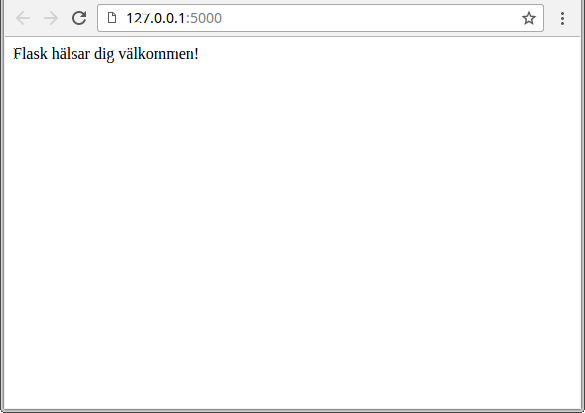
\includegraphics[width = \linewidth]{flask_test_server.png}
    \caption{Flask server test}
    \label{fig:flask_server}
\end{figure}
Om ovanstående ej fungerar, se sektion 4.2


\newpage
\section{Felsökning och underhåll}
\subsection{Logging}
Logging av varje anrop till programmet sparas på en separat textfil(Logg.txt). Denna fil hittar du i samma mapp som programfilen är placerad i.

I loggen visas information såsom tid för anrop, vilka parametrar skickades in med anropet och vilka parametrar skickades ut. Här kan även den sökväg på källfilen där logganropet skedde i och funktionsnamnet som innehåller loggningsanropet visas. Utöver detta kan kodraden som loggningsanropet skedde på också visas. Eventuella felmeddelanden som uppstår skrivs också i loggfien. Varje loggmedelande får var sin flagga för att visavilken typ av meddelande det är (se tabell \ref{fig:logging_flags}).

\begin{table}[!h]
\caption{Flaggor för loggmeddelanden.}
\label{fig:logging_flags}
\begin{tabularx}{\linewidth}{|l|X|}
\hline
Flagga & Innebörden av flaggan 
\\ \hline
INFO & Anropet har skett utan problem. 
\\ \hline
ERROR & Något har gått snett men programmet kan fortsätta. 
\\ \hline
CRITICAL & Ett fel som orsakar att programmet ej kan fortsätta. 
\\ \hline
\end{tabularx}
\end{table}

\subsection{Debugging}
Om det inte fungerar att starta din server, kan du starta Flasks debugger. Detta gör du me hjälp av denna kod:
\begin{lstlisting}[language=bash]
export FLASK_DEBUG=1
flask run
\end{lstlisting}
Här kan du gå igenom koden och få mer information om varför det inte gick att starta servern.

\end{document}
